\documentclass[12pt]{article}

\usepackage[a4paper,margin=2.5cm]{geometry}
\usepackage{amsmath, amssymb, amsthm}
\usepackage{bm}
\usepackage{hyperref}
\usepackage{graphicx}
\usepackage{caption}
\usepackage{listings}
\usepackage{xcolor}
\usepackage{float}
\usepackage{placeins}
\graphicspath{{figures/}}

\lstdefinestyle{code}{
  basicstyle=\ttfamily\small,
  numbers=left,
  numberstyle=\tiny,
  numbersep=8pt,
  keywordstyle=\color{blue},
  commentstyle=\color{teal!70!black},
  stringstyle=\color{orange!70!black},
  showstringspaces=false,
  breaklines=true,
  frame=single,
  framerule=0.3pt,
  rulecolor=\color{black!15}
}
\lstset{style=code}

\title{K-means Clustering Tutorial}
\author{}
\date{\today}

\begin{document}
\maketitle

\section{Introduction}
K-means clustering partitions observations into \(K\) disjoint groups by minimizing within-cluster variance. The algorithm alternates between assigning each point to its nearest centroid and updating centroids as the mean of assigned points. Because K-means assumes roughly spherical clusters of similar density, it performs best on standardized numeric features and can struggle with elongated or irregular shapes.

\section{Theory and Formulas}
\subsection{Objective Function}
Given data matrix \(\mathbf{X} = [\mathbf{x}_1,\dots,\mathbf{x}_n]^\top\), K-means minimizes
\begin{equation}
\min_{\{C_k\},\{\bm{\mu}_k\}} \sum_{k=1}^K \sum_{\mathbf{x}_i \in C_k} \lVert \mathbf{x}_i - \bm{\mu}_k \rVert_2^2,
\end{equation}
where \(C_k\) denotes the index set of cluster \(k\) and \(\bm{\mu}_k\) its centroid. This is equivalent to maximizing between-cluster dispersion when total dispersion is fixed.

\subsection{Lloyd's Algorithm}
The iterative refinement procedure typically used is:
\begin{enumerate}
  \item \textbf{Initialization}: choose \(K\) starting centroids, often via k-means++ to promote separation.
  \item \textbf{Assignment}: allocate each point to the cluster with the nearest centroid under the chosen distance metric (commonly Euclidean).
  \item \textbf{Update}: recompute each centroid as the mean of its assigned points.
  \item Repeat steps 2--3 until assignments stop changing or the centroid shifts fall below a tolerance.
\end{enumerate}
Although convergence is guaranteed, it may reach a local minimum, so multiple restarts with different seeds are recommended.

\subsection{Relationship to Variance Decomposition}
K-means implicitly minimizes the trace of within-cluster scatter matrix \(\mathbf{S}_W\). For standardized data, total scatter \(\mathbf{S}_T\) decomposes as \(\mathbf{S}_T = \mathbf{S}_W + \mathbf{S}_B\), with between-cluster scatter \(\mathbf{S}_B\) capturing centroid separation. Lower within-cluster inertia therefore corresponds to higher between-cluster separation.

\section{Applications and Tips}
\begin{itemize}
  \item \textbf{Customer segmentation}: group customers by purchasing patterns or engagement metrics to tailor marketing strategies.
  \item \textbf{Vector quantization}: compress signals or images by mapping observations to a limited set of prototype vectors.
  \item \textbf{Feature engineering}: use cluster IDs as categorical features for downstream supervised models.
  \item \textbf{Best practices}: scale features, inspect inertia and silhouette for model selection, and watch out for sensitivity to outliers.
\end{itemize}

\section{Python Practice}
The script \texttt{gen\_clustering\_k\_means\_figures.py} synthesizes three Gaussian blobs, applies K-means, and saves both the labeled scatter plot and an elbow curve of inertia versus \(K\).
\begin{lstlisting}[language=Python,caption={Excerpt from gen_clustering_k_means_figures.py}]
from sklearn.cluster import KMeans

kmeans = KMeans(n_clusters=3, init="k-means++", n_init=10, max_iter=300,
                random_state=42)
labels = kmeans.fit_predict(points)

inertias = []
for k in range(1, 9):
    model = KMeans(n_clusters=k, init="k-means++", n_init=10,
                   max_iter=300, random_state=42)
    model.fit(points)
    inertias.append(model.inertia_)
\end{lstlisting}

\section{Result}
\begin{figure}[H]
  \centering
  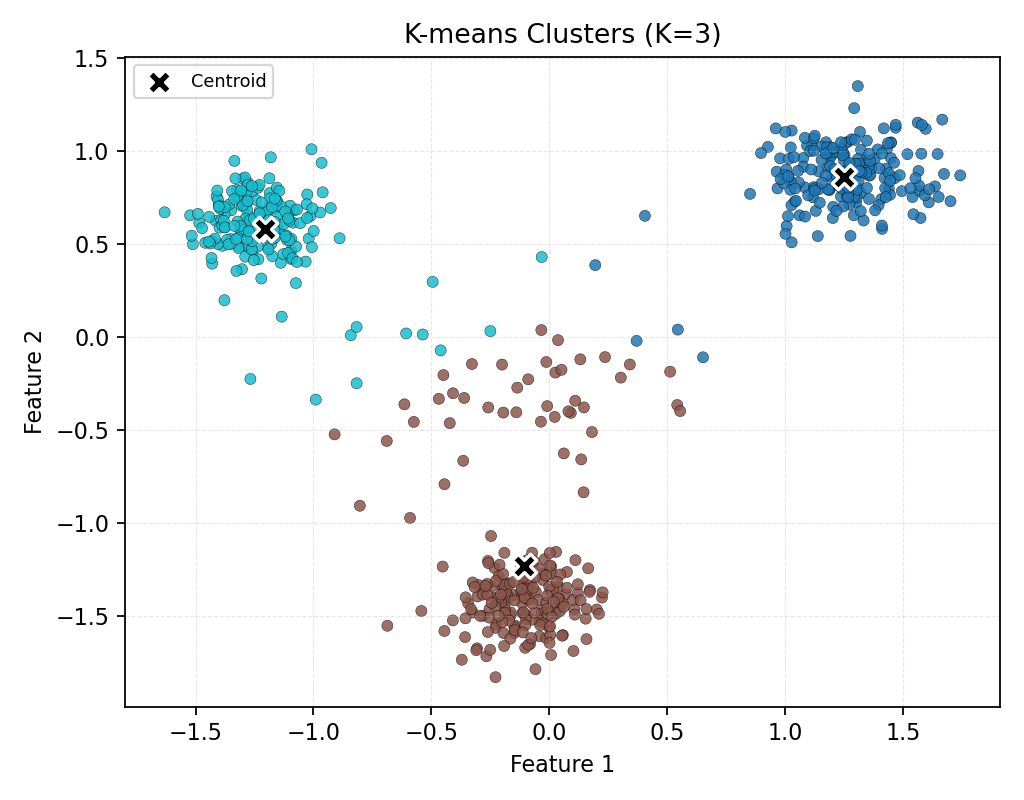
\includegraphics[width=0.8\linewidth]{kmeans_clusters.png}
  \caption{K-means clustering of synthetic blobs (\(K=3\))}
  \label{fig:kmeans_clusters}
\end{figure}

\begin{figure}[H]
  \centering
  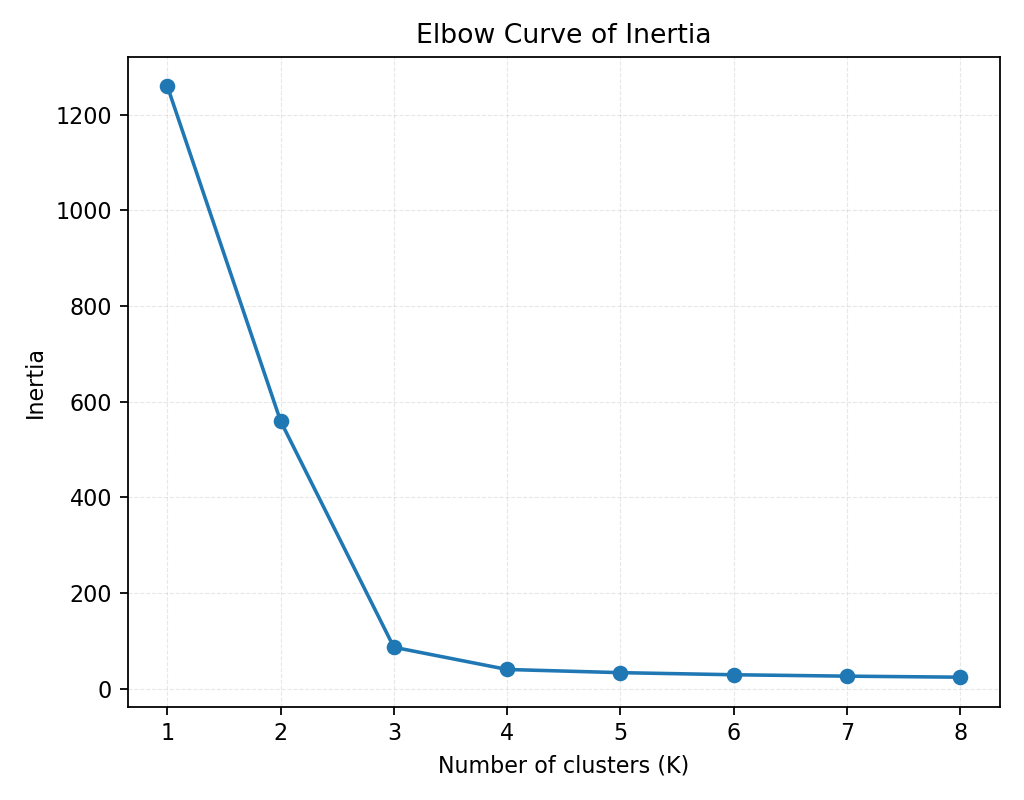
\includegraphics[width=0.8\linewidth]{kmeans_elbow.png}
  \caption{Elbow curve of inertia versus number of clusters}
  \label{fig:kmeans_elbow}
\end{figure}

\FloatBarrier
\section{Summary}
K-means offers a fast and scalable method for partitioning standardized numeric data when clusters are roughly spherical. Proper initialization, multiple restarts, and diagnostic plots such as the elbow method help mitigate local minima and over- or under-segmentation. The synthetic example demonstrates a typical workflow from clustering to inertia analysis.

\end{document}
